\documentclass{article}
\usepackage[utf8]{inputenc}
\usepackage{amsmath}
\usepackage{amsthm}
\usepackage{amssymb}
\usepackage[margin=1.0in]{geometry}
\usepackage{multirow}
\usepackage{tikz}
\usepackage{hyperref}
\usepackage{enumitem}
\usepackage{caption}
\usepackage{subcaption}
\usepackage{csvsimple}
\hypersetup{
    colorlinks=true,
    linkcolor=blue,
    filecolor=magenta,      
    urlcolor=cyan,
    pdftitle={Overleaf Example},
    pdfpagemode=FullScreen,
    }
\def\checkmark{\tikz\fill[scale=0.4](0,.35) -- (.25,0) -- (1,.7) -- (.25,.15) -- cycle;}
\usepackage[english]{babel}
\usepackage{graphicx}
\graphicspath{ {images/} }
\newtheorem{theorem}{Theorem}[section]
\newtheorem{corollary}{Corollary}[theorem]
\newtheorem{lemma}[theorem]{Lemma}
\DeclareMathOperator{\GCC}{GCC}
\DeclareMathOperator{\sign}{sign}

\title{Greedy Approaches utilizing Centrality for Node-Weighted Network Dismantling}
\author{Alex Sanchez, Anthony Maltsev, Rishi Nath}
\date{May 7th, 2023}

\begin{document}

\maketitle

\begin{abstract}
    
\end{abstract}
Our study is centered around the use of centrality to develop greedy algorithms for the network dismantling problem, which is NP-complete. 
In graph theory, network dismantling refers to the problem of identifying a set of vertices whose removal would break the graph into connected components of at most a given target size. 
In our study, we do a survey of existing network dismantling algorithms and heuristics for node-weighted graphs. 
We also suggest new approaches to modifying unit-case centrality heuristics to the node-weighted case. 
Finally, we implement many of our surveyed and suggested approaches to compare their performance on a diverse set of node-weighted graphs. 
We also introduce a new scoring method for generalized network dismantling algorithms called weighted robustness.
\newpage

\section{Introduction and Motivation}
 \null\quad In graph theory, network dismantling refers to the problem of identifying a set of vertices whose removal would break the graph into connected components of at most some constant size, $C$. 
 This problem is well-motivated by real world issues. One example is the issue of criminal network dismantling: law enforcement agencies may wish to break up a large criminal network by arresting some key members \cite{tostado2022human}. 
 Another example would be figuring out a set of social media users which could be banned to break up online hate groups. 
 The problem is also relevant in terms of network designs: if the cost to dismantle a network is high then one can consider that network to be secure.
 This is applicable to power grids or public transport networks which aim to have high connectivity or uptime. \\
 \null\quad Network dismantling is known to be in the class of NP-complete problems. This is shown by a reduction from vertex cover, which is also NP-complete \cite{braunstein}. 
 Thus, the problem of finding an exact solution to network dismantling is a computationally intractable problem and research in the area is focused on developing heuristic algorithms that perform well on representative graphs (ER graphs or real-life networks such as Twitter). 
 As Braunstein et al \cite{braunstein} note, the optimal solution to network dismantling is inherently collective: the optimal solution is not necessarily comprised of vertices that perform well individually. 
 Nonetheless, state-of-the-art algorithms that perform well in practice are often greedy in some way.
 Many modern algorithms can be broken into two classes: 1.) removing individual nodes greedily according to some measure of centrality, and 2.) iteratively removing some subset of nodes in a greedy way until the condition is satisfied. \\
 \null\quad In this paper, we will focus on the generalized problem of network dismantling in which nodes can have arbitary nonnegative weights.
 Dismantling node-weighted graphs is also well-motivated: for instance, in the case of criminal networks, the weight of a node may be representative of the difficulty of arresting a given actor \cite{covert}.
 However, literature on node-weighted network dismantling is limited at best \cite{gnd}. 
 We will review some state-of-the-art algorithms for network dismantling. 
 In an attempt to contribute to the node-weighted network dismantling literature, we will adapt commonly-used heuristics to fit node-weighted networks. Additionally, we will also propose and test some new centrality measures of our own.


\section{Problem Definition}

\null\quad We will now formally define the problem of network dismantling and generalized network dismantling. Let us define $\GCC(G)$ as the number of vertices in the largest connected component of graph $G = (V,E,W)$. Let us define a set $D$ of subsets of vertices such that removing those vertices will dismantle the graph: $D = \{ S : \GCC((V', E', W)) \leq C \}$ where $V' = V \setminus S$, $E' = E \setminus \{ (u,v) \in E : u \in S \vee v \in S \}$, and $C$ is a known parameter. Then, network dismantling is the problem of finding the element $S \in D$ of minimal size $|S|$. Generalized network dismantling is the problem of finding the element $S \in D$ that minimizes total weight $\sum_{v \in S} W(v) \triangleq W(S)$. See \ref{fig:dismantling example} for an example of a graph and a dismantling set for that graph.

\begin{figure}[h]
    \centering
    \begin{subfigure}[b]{0.4 \textwidth}
        \centering
        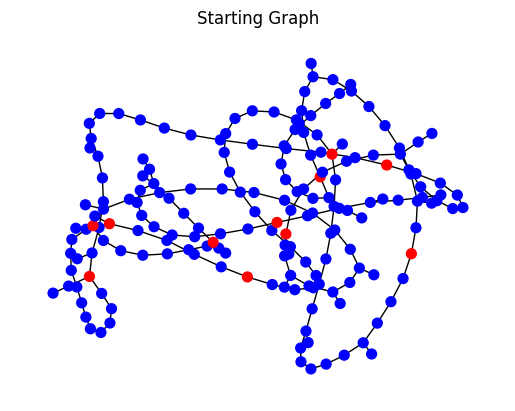
\includegraphics[width=\textwidth]{starting_graph_example.png}
        \label{fig:starting}
    \end{subfigure}
    \begin{subfigure}[b]{0.4 \textwidth}
        \centering
        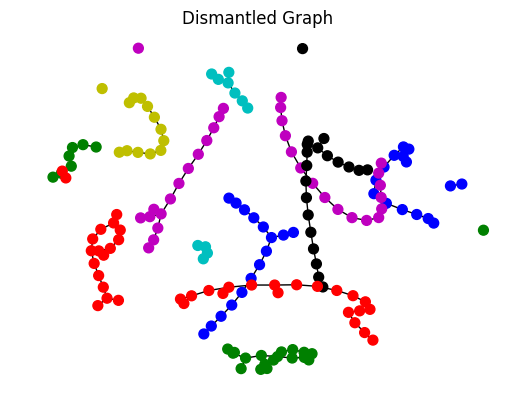
\includegraphics[width=\textwidth]{dismantled_graph_example.png}
        \label{fig:dismantled}
    \end{subfigure}
    \caption{Left: Starting Graph with an example dismantling set found by approximate betweenness centrality (ABS) with $\log{n}$ pivots, labeled in red. Right: The resulting graph upon deletion of the dismantling set, colored by connected components.}
    \label{fig:dismantling example}
\end{figure}
% \newpage % TODO: I added this for formatting purposes. if the layout changes this might not be needed

\section{Existing Algorithms}
\null\quad There are many existing competitive algorithms for network dismantling with unit removal costs. 
For the generalized network dismantling problem, however, the literature is much less comprehensive. 
In this section, we will present an overview of some state-of-the-art algorithms for network dismantling.
Many of these algorithms perform similarly for networks with unit costs, so we will first give a brief overview of some algorithms for nodes with unit cost. 
Then, we will cover the Generalized Network Dismantling algorithm, which we will use later to benchmark other algorithms.

\subsection{Min-Sum}
The Min Sum algorithm, introduced by Braunstein et al. \cite{braunstein}, is an algorithm for network dismantling with unit removal costs. 
The algorithm is composed of three main steps: 1.) decycle the graph, 2.) break trees, and 3.) greedily reinsert cycles into the graph. 
The decycling step is done through the a method inspired by the Min Sum algorithm for low density parity checking in message decoding, hence the name of the algorithm. 
The greedy reintroduction of cycles is done by iterating through all nodes removed in the decycling stage and reinserting the one which increases the GCC of the graph by the smallest amount until no more nodes can be reinserted. 

\subsection{Equal Graph Partitioning}
The Equal Graph Partitioning algorithm introduced by Chen et al \cite{egp} approaches network dismantling by attempting to split the graph into equally sized connected components. 
The main idea of the algorithm is based on the nested dissection algorithm -- a method primarily used to solve sparse systems of linear equations quickly by modeling the system of equations as a graph and splitting that graph into equally sized components. 
EGP's implementation of nested dissection allows a split of a graph into an arbitrary ratio of size (e.g. into two connected components of size 2:1). 
They recursively dissect each connected component until the graph is sufficiently dismantled. 

\subsection{Generalized Network Dismantling}
\subsubsection{Algorithm}
Generalized network dismantling (GND) is an algorithm developed by Ren et al \cite{gnd} that uses iterative spectral bisection to dismantle a graph. 
In more detail, GND repeatedly looks at the greatest connected component of the graph and tries to find the minimal weight bisecting cut for that connected component until the size of the greatest connected component is $\leq C$. 
The weight of the cut is determined by the edges crossing the cut. 
This motivates a conversion from node weights to edge weights so that the minimal weight cut can be covered by removing a minimally weighted set of vertices adjacent to the cut edges. 
Specifically, the weight of each edge $e = (u,v)$ to be $w_e = W(u) + W(v) - 1$. Then, the weighted adjacency matrix $B = AW + WA - A$ and the node-weighted Laplacian matrix $L_w$ is calculated based on this weighted adjacency matrix. 
The minimal weight bisecting cut is found by the following optimization problem:
$$\begin{array}{cc}
    \min_v & \frac{1}{4}v^TL_wv \\
     & \\
    \text{s.t.} & \mathbf{1}^Tv = 0 \\
     & v_i \in \{-1, 1\}
\end{array}$$
Here $v_i = 1$ would represent being in set $S$ and $v_i = -1$ represents being in set $\bar{S}$. 
This optimization problem is intractable, so the final constraint is relaxed to $v_i \in \mathbb{R}$. 
Under this relaxation, set membership is determined by $\sign(v_i)$. 
By the Courant-Fischer theorem, this relaxed optimization problem has an analytic solution in $v_2$, the second eigenvector of the weighted Laplacian $L_w$. \\

Having found a bisecting cut, we need to choose some set of vertices along that cut whose removal will remove all edges across the cut. 
This is done by simply applying a weighted vertex cover approximation algorithm to the subgraph along the cut. 
A repeated application of these steps will dismantle the graph.
\subsubsection{Complexity}
The complexity of generalized network dismantling is highly dependent on the complexity of finding the second eigenvector of the Laplacian. Naïvely computing the spectral decomposition to find the second eigenvector would yield a runtime worse than $\Omega(n^2)$ (the runtime of matrix multiplication). 
Ren et al. \cite{gnd} introduce a faster approximation algorithm for computing the second eigenvector of the Laplacian. This is based on a power iteration method. 
First, you draw a point from the unit sphere at random and take the component orthogonal to the first eigenvector ($\mathbf{1}$). 
Call this vector $v$. 
Then, repeat $v \leftarrow \frac{\tilde{L}v}{||\tilde{L}v||_2}$ for $\eta(n)$ iterations where $\Tilde{L} = 6d_{max}I_n - L_w$ and $d_{max}$ is the maximal degree in the graph. 
So long as $\eta(n)$ grows faster than $\frac{11}{2\log(\frac{|\tilde{\lambda_2}}{|\tilde{\lambda_3}|})} \log(n)$ then this approximation will almost surely converge to $v_2$. 
A proof of this is provided in the appendix of \cite{gnd}. 
The runtime of this approximation is then $\mathcal{O}(\eta(n)n) = \mathcal{O}(n\log^{1+\epsilon}(n))$. By Master's Theorem, the total runtime of running this approximation recursively on every connected component until the graph is completely dismantled is given by $\mathcal{O}(n\log^{2+\epsilon}(n))$.

\subsubsection{Performance}
Experimental analysis from \cite{gnd} shows that GND performs about as well as other state of the art methods for the unit-weight case. 
With the inclusion of node-weights, GND outperforms other algorithms that do not include weights. 
The performance of GND can be improved by including a greedy reinsertion step at the end, as in the Min Sum algorithm of \cite{braunstein}.
In our experiments, however, we do not perform this greedy reinsertion at the end.


\section{Centrality in Network Dismantling}
 When looking at a graph, it can be easy to tell what nodes are important holistically. For example, a node with high degree is probably important. Similarly, a single node which connects two otherwise disconnected but large components is also probably important. A centrality measure is a well-defined \textbf{measure} which seeks to quantify this importance. 
 
 Different centralities seek to measure different definitions of importance. One measure of importance is \textbf{radial} importance - if a node is connected to many other nodes, for example, a city center or a leader, it is radially central. 
 Alternatively, \textbf{medial} importance highlights critical connections in infrastructure, which if removed would disconnect a network. Obviously, in the context of network dismantling, we are more interested in the latter. 
 Also, centralities that measure \textbf{length} are related to closeness and measure the length of paths travelling through a node, while centralities measuring \textbf{volume} measure the amount of paths travelling through a node. Again, we are more interested in the latter.
 
 Imagine we had a good centrality measure, which told us which node is most critical node vulnerable to removal for any network. 
 We can define a greedy algorithm which repeatedly uses this measure to remove vertices until the greatest connected component (GCC) is smaller than our target size $C$. 
 Much work has been done with greedy algorithms using centrality for the unweighted (unit case) network-dismantling problem \cite{analysis}. 
 In this study, we seek to find, define, and evaluate multiple centrality measures on their usefulness in the \textit{node-weighted} network dismantling problem.

 A greedy approach with betweenness centrality has been shown to perform well experimentally for unit removal costs. This motivates the question of whether there are other good centrality measures for network dismantling. While much work has been done both for the network dismantling problem, and also much work has been done in the study of centrality, node-weighted network dismantling and node-weighted centrality are both areas of study with little work. We compare our work to Generalized Network Dismantling (GND) developed by Ren et al. \cite{gnd}, which is one of the few published algorithms on node-weighted network dismantling. Thus, we also seek to find meaningful definitions for centrality on node-weighted graphs for each of the centrality measures we cover.


\subsection{Degree Centrality}
Degree centrality is the simplest and most intuitive measure of node centrality. 
The degree centrality of a node $u$ is simply its degree. 
The weighted degree centrality of $u$ is its weighted degree, which is defined as $$ DC_{\text{weighted}}(u) = \sum_{v \in V} a_{u,v} \cdot w_v $$ where $a_{u, v}$ is 1 if $(u, v) \in E$ and 0 if not. 
In other words, it is an entry in the adjacency matrix of $G$

\subsubsection{Network Dismantling}
Intuitively, a greedy dismantling algorithm using degree centrality performs well on highly connected graphs with homogeneous node weights. This is because on these kinds of graphs, the problem of dismantling is really just removing nodes one by one from the main component, as there are not different 'communities' of nodes to disconnect from each other. However, degree centrality is not very competitive for network dismantling for real-world networks \cite{analysis}, as they are typically not homogeneous or highly connected. 
We still use degree centrality as a baseline and a sanity check when developing other measures of centrality, though.

\subsubsection{Centrality Density}
Note that the weighted degree centrality of a node $u$ does not take into account $w_u$, or the node's own weight. Because the neighbors of $u$ do take $w_u$ into account, and we only care about the relative ordering of centralities, this is not a concern. However, for greater control, we introduce the concept of Centrality Density (CD). Simply, we divide the centrality of each node by its weight to the power of a tuning parameter $\alpha$.

$$DC_{\text{CD, weighted}}(u) = \frac{DC_{\text{weighted}}(u)}{{w_u}^\alpha}$$

CD will be used to help define other measures of centrality in terms of node-weighted centrality. We only used $\alpha=1$ in our testing, but in practical applications, it may be useful to find a better $\alpha$ as the optimal relation may not be linear. $\alpha$ can also be set to a negative number, in situations where weight is a reward instead of a cost, though that is out of the scope of this project.
In order to simplify notation, we will write only $CD$, for both the weighted and unweighted case, as long as it is clear from context which one we are referring to.

\subsection{Betweenness Centrality}
Betweenness centrality is a measure based on the shortest paths between different pairs of nodes \cite{BRANDES2008136}.
In this centrality measure, nodes that appear more often in shortest paths are weighted more highly.
Intuitively, this is intended to be reflect that nodes that act as "bridges" between other nodes are more important than those that do not.

\subsubsection{Definition}
We now proceed to define betweenness centrality more formally.
Let $SP_{st}$ denote the set of shortest paths between a source node, $s$, and a target node, $t$. 
Similarly, consider the set $SP_{st}(v)$, which is the set of shortest paths between $s$ and $t$ such that $v$ is a part of the path.
We also define $\sigma_{st} := |SP_{st}|$ and $\sigma_{st}(v) := |SP_{st}(v)|$.
Then, the betweenness centrality for any given node, $v \in V$ is:
$$BC := \sum\limits_{s, t \in V}\frac{\sigma_{st}(v)}{\sigma_{st}}$$

\subsubsection{Node Weighted Approaches}
We consider three approaches to modifying BC for node-weighted graphs.
\begin{enumerate}[label=\textbf{\Alph*}.]
\item \textbf{Centrality Density BC:} We define $BC_{CD}(u) = \frac{BC_{CD}(u)}{w_u^\alpha}$. As explained in 4.1.2, centrality density allows us to consider the cost of removing the node $u$.
\item \textbf{Weighted Shortest Path BC:} We define a simple transformation from node weights to edge weights. For every edge $e = (u, v)$ define $w_e = \frac{1}{(w_u + w_v)^\beta}$, where $\beta$ is a tuning parameter. This sets the strength of each link to the sum of its endpoints, which is a standard transformation. Then, we calculate edge-weighted betweenness centrality on this graph, which is defined by Brandes \cite{BRANDES2008136}. This is useful for dismantling because it is helpful to disconnect costly nodes. This approach can also be combined with CD.
\item \textbf{Weighted Endpoints BC:} As suggested by Singh et. al. \cite{singh}, a useful way to define weighted betweenness centrality is to multiply the shortest-paths ratio with a function of the endpoints used. We define $BC_{\text{WEndp}}(u) = \sum_{s,t}(w_s + w_t)^\gamma \cdot {\frac{\sigma_{st}(u)}{\sigma_{st}}}$, where $\gamma$ is a tuning parameter. This also places importance on disconnecting costly nodes. This approach can also be combined with CD.
\end{enumerate}

\subsubsection{Network Dismantling}
It has been shown that betweenness centrality is notably excellent and usually yields the best dismantling sets out of any algorithm on unit cases \cite{analysis}. 
Our own results confirm that it also performs remarkably on the node-weighted dismantling problem. However, since it requires computing all pairs of shortest paths, it is prohibitively slow, timing out on most of the larger graphs in our experiments.

\subsubsection{Complexity}
Betweenness centrality can be calculated in $\mathcal{O}(nm)$ time on unweighted graphs using Brandes's algorithm \cite{betweennessfast}. 
Thus, if we use BC in a greedy network dismantling algorithm, which has at most $n$ iterations, the runtime is $\mathcal{O}(n^2m)$, which is quite slow. Given that most interesting, real-life networks have a large number of nodes, the computation of BC can become a prohibitive operation.
There also exists algorithms to approximate betweenness centrality (ABC) \cite{abc}, the simplest of which instead of considering all possible s-t paths, considers $\log{n}$ s-t paths sampled uniformly at random.

\subsection{Current-Flow Betweenness Centrality}
Current-Flow is an approach to network analysis based on facts about the flow of current in electrical circuits developed by Brandes et al. Current-flow betweenness centrality (CfBC) is an application of this analysis applied to traditional betweenness centrality. The CfBC of a node $u$ is related to the proportion of current flowing through it. CfBC is also called \textit{random-walk betweenness}, as it is also related to the expectation of random st-walks. It is also closely related to information centrality (current-flow closeness centrality is equivalent to information centrality) \cite{current}.

It is also interesting to note that the Laplacian of a matrix can be calculated by applying Kirchoff’s Current Law to create a representative matrix, and then multiplying that matrix by its own transpose. This means that current-flow analysis is closely tied with the properties of the Laplacian.

\subsubsection{Definition}
This is an abbreviated version of the definition and derivation in the Appendix. We  define the \textit{throughput} $\tau$ of a node $u$ to be the sum of the absolute value of the currents $x$ through $u$. The current $x(\Vec{e}=(u,v))$ through an edge is related to that edge's \textit{resistance} (the inverse of its weight) and that edge's \textit{potential difference} $p_{st}(u) - p_{st}(v)$. Potential differences are defined in terms of a \textit{s-t flow}, where vertex $s$ is a \textit{supply} of 1 unit of current, and vertex $t$ is a \textit{sink} of 1 unit of current. We define current-flow betweenness centrality (CfBC) to be: $$ \text{CfBC}(u) = \sum_{s,t \in V} \tau_{st}(v)$$
\\\\
It is also useful to define $x(\Vec{e})$ in matrix notation. We define an incidence matrix $B$, where $B_{ve} = c(e)$ if $\Vec{e} = (v, \cdot$), $= -c(e)$ if $\Vec{e} = (\cdot, v$), or $= 0$ otherwise. Define $F = BC$, where C is the inverse simplified Laplacian which solves $p = C b$. It can be shown that $x_{st}(\Vec{e}) = F_{es} - F_{et}$.
\subsubsection{Network Dismantling}
CfBC is intuitively similar to betweenness centrality (BC). However, BC only considers shortest paths, while we care about connectivity, which is broader than shortest paths. Network flow possibly better represents important connections.

\subsubsection{Node-weighted Approaches}
We present and test four (technically, 7) approaches to modifying CfBC for node-weighted graphs.
\begin{enumerate}[label=\textbf{\Alph*}.]
\item \textbf{Centrality Density CfBC:} $\text{CfBC}_{CD}(u) = \frac{\text{CfBC}(u)}{{w_u}^\alpha}$, similar to CD approaches shown above.
\item \textbf{Weighted Edge  CfBC:} We define a simple transformation from node weights to edge weights. For every edge $e = (u, v)$ define $w_e = \frac{1}{(w_u + w_v)^\beta}$, where $\beta$ is a tuning parameter. This sets the resistance of each edge to the sum of its endpoints. This is an accurate measure on how importance would flow through the graph based on node weights though a current-flow analysis. Thus, simply calculate Brandes' CfBC on this graph. This can also be combined with the CD approach.
\item \textbf{Weighted Supply CfBC:} When considering a particular \textit{st-path} in the calculation of CfBC, instead of choosing unit supplies and sinks, we supply current based on the sum of the weights of the endpoints $(w_s + w_t)^\gamma = k_{st}$, where $\gamma$ is a tuning parameter. This approach places higher importance on nodes which conduct current between two expensive nodes, as it is beneficial to disconnect them. We derive in the Appendix that this is found by
$ 
\text{CfBC}_{\text{WSup}} = \sum_{s,t} k_st \cdot \tau_{st}(v)
$
where $\tau_{st}(v)$ is still calculated with unit $b$.
\item \textbf{WEdge \& WSup CfBC:} Finally, we can combine Weighted Edge and Weighted Supply, and also optionally CD. Note that we have three seperate tuning parameters $\alpha, \beta, \gamma$, though in this study we only consider $\alpha = \beta = \gamma = 1$.
\end{enumerate}

\subsubsection{Complexity}
The complexity of CfBC is dominated by inverting the Laplacian. Certain speedups exist for inverting a sparse Laplacian, which improve the runtime from $\mathcal{O}(n^3)$ to $\mathcal{O}(nm  \sqrt{k} mn \log{n})$ where $k$ is the Laplacian matrix condition number, though this cannot be applied to all graphs. Thus, if we use CfBC in a greedy network dismantling algorithm, which has at most $n$ iterations, the runtime is $\mathcal{O}(n^4)$, which is extremely slow on real-world networks.

We can also approximate current-flow betweenness, which runs in $\mathcal{O}(\epsilon^{-2} m \sqrt{k} \log{n})$ which approximates current-flow betweenness with an error of epsilon with high probability, where k is the maximum amount of s-t flows we consider per iteration \cite{current}. Thus, if we use approximated CfBC in a greedy network dismantling algorithm, which has at most $n$ iterations, the runtime is $\mathcal{O}(\epsilon^{-2} nm \sqrt{k} \log{n})$.

\subsection{Eigenvector Centrality}

Eigenvector centrality is a measure of node importance in a network based on the idea that a node is important if it is connected to other important nodes. A node’s eigenvector centrality is proportional to the sum of its neighbors' eigenvector centrality. Thus, a node with high eigenvector centrality means that it is connected to important nodes \cite{bonacich}.
Importantly, a node with few, but important, connections may have higher eigenvalue centrality than a node with many, but less important connections.

Eigenvector centrality measures the influence a node has in the network. It can also be seen as measuring not only direct connections, but indirect connections of all lengths, thus measuring influence over the entire network \cite{bonacich2}.

\subsubsection{Definition}
Formally, eigenvector centrality for a node $u$ can be defined as $$ EC(u) = c \cdot \sum_{v \in V} a_{u,v} \cdot EC(v)$$ This is notably similar to degree centrality, with the difference that each vertex also considers the importance of its neighbors \cite{singh}. The constant $c$ can be chosen arbitrarily for convergence because we only care about the ordering of the centralities. 

Note that this is a recursive definition. For a graph with $n$ nodes, say the vector $\Vec{x} \in \mathbb{R}^n$ represents the eigenvector centrality of each node. With the adjacency matrix of the graph \textbf{A}, we can define the vector $\Vec{x}$ to be $$\Vec{x} = c \cdot \textbf{A} \Vec{x}$$ Note that this is the same definition as above, just in matrix-vector notation. Clearly, this converges if $\Vec{x}$ is chosen to be an eigenvector of \textbf{A}, and $c$ the inverse of the corresponding eigenvalue. We can use power iteration [foot note explaining power iteration] to find the eigenvector corresponding to the largest eigenvalue relatively quickly, as we do not require a high degree of precision.

\subsubsection{Network Dismantling}
Eigenvector centrality is useful for network dismantling because eigenvector centrality measures a degree of mediality. Consider three nodes in a line, where the nodes on each end are heavily connected while the node in the middle only connects those two. With eigenvector centrality, the centrality of the connector node in the middle will be increased by both the centralities of its neighbors. Thus, eigenvector centrality is medial, which is useful for network dismantling.

\subsubsection{Node-weighted Approaches}
Eigenvector centrality is uniquely challenging to meaningfully define for node-weighted graphs because its definition is dependent upon the eigenvectors of the adjacency matrix, which is unweighted \cite{singh}.
We propose and test three approaches to defining eigenvector centrality on node-weighted graphs.
\begin{enumerate}[label=\textbf{\Alph*}.]
\item \textbf{Centrality Density EC:} The naive CD approach for eigenvector centrality is to ignore node weights in the calculation, and simply divide the unweighted eigenvector centrality by the node weight for each node, to the power of a tuning parameter alpha. The issue with this approach is that node weights are ignored in the eigenvector centrality calculation, meaning the centrality measure itself is unaware of the importance of nodes based on their node weight.
\item \textbf{Weighted Matrix EC:} In the network dismantling problem, nodes with larger weights are more costly to remove. However, we can also say that it is better if we disconnect two nodes with large weights. Thus, it would be useful if we could capture the notion of being connected to highly weighted nodes. Motivated by this, we can define node-weighted eigenvector centrality to be dependent (with tuning parameter $\beta$) on the node weights: $$ EC_{\text{WMat}}(u) = c \cdot \sum_{v \in V} {w_v}^\beta \cdot a_{u,v} \cdot EC(v) $$ Following algebraically from this, we are now interested in the \textit{weighted adjacency matrix} of G. The matrix-vector form of this approach is $$ \Vec{x} = c \cdot {A_W}^{\beta} \Vec{x} $$ where $A_W$ is the weighted adjacency matrix. 
We can also combine this approach with CD.
\end{enumerate}

\subsubsection{Complexity}
The runtime complexity of calculating eigenvector centrality is dominated by the eigenvector calculation. Using power iteration to calculate the eigenvector yields a runtime of $\mathcal{O}(n)$ \cite{gnd}, as we do a matrix-vector multiplication a constant number of times. Thus, if we use eigenvector centrality in a greedy network dismantling algorithm, which has at most $n$ iterations, the runtime is $\mathcal{O}(n^3)$. 

\subsection{Laplacian Centrality}
\subsubsection{Definition}
Laplacian Centrality is a centrality measure that is related to the contribution of an individual node to the spectrum of the Laplacian matrix associated with a graph. The measure is defined for edge-weighted graphs. Laplacian Centrality was introduced by Qi et al in \cite{laplacian}. The measure is motivated as an intermediate between radial measures like degree and medial measures like betweenness. Some intuition for the definition of this measure is that the spectrum of the Laplacian acts as a measure of connectivity in itself: for instance the second eigenvalue detects whether the graph is connected and its magnitude indicates how connected the graph is. Let us define, following \cite{laplacian}, some quantities relevant to the measure. With $\{\lambda_i\}$ as the eigenvalues of the Laplacian matrix, let the Laplacian energy $E_L(G)$ of a graph be:
$$E_L(G) \triangleq \sum_{i=1}^n \lambda_i^2$$
Then, the Laplacian centrality $C_L(v_i, G)$ of the node $v_i$ is defined as the change in Laplacian energy when $v_i$ is removed from the graph:
$$C_L(v_i, G) \triangleq \frac{\Delta (E_L(G))_i}{E_L(G)} = \frac{E_L(G) - E_L(G \setminus v_i)}{E_L(G)}$$
% Let us denote $x_i$ as the sum of edge weights incident to node $v_i$: $x_i = \sum_{e=(i,v) \in E}w_e$. Interestingly, by analyzing the characteristic polynomial of the Laplacian matrix, an alternate form of the Laplacian Energy arises:
% $$E_L(G) = \sum_{i=1}^n x_i^2 + 2\sum_{i < j} w_{(i,j)}$$
% Using this formulation of Laplacian energy, one can compute that the change in Laplacian energy due to removing node $v_i$, $\Delta (E_L(G))_i$
In \cite{laplacian}, it is shown that $C_L$ can be expressed as a function of the number of 2-length walks that pass through $v_i$:
$$C_L(v_i,G) \propto 2\cdot NW_2^E(v_i) + 2 \cdot NW_2^M(v_i) + 4 \cdot NW_2^C(v_i)$$
Here, $NW_2^E(v_i)$ refers to the number of length 2 paths in the graph where one of the endpoints is $v_i$ (i.e. a path of the form $v_k \to v_l \to v_i$). Similarly, $NW_2^M(v_i)$ refers to the number of walks length 2 paths in the graph where the middle vertex is $v_i$ (i.e. a path of the form $v_k \to v_i \to v_l$). $NW_2^C(v_i)$ refers to the number of length 2 paths where the middle vertex is $v_i$ and the path is closed (i.e. a path of the form $v_k \to v_i \to v_k$). A proof of this fact, relying on an alternate expression of the Laplacian energy as a function of degrees and edge weights, appears in \cite{laplacian}. \\

Then, the Laplacian centrality of a node is based entirely on the neighborhood of nodes within a distance of 2 edges to that node. In this sense, one can think of Laplacian centrality as a more inclusive version of degree centrality: it is a mostly radial measure that considers the connectivity of a node to the neighborhood near it.

\subsubsection{Network Dismantling}
As a mostly radial centrality measure, Laplacian centrality does not function as a great measure of the influence of a node on the connectivity of a graph. For networks of small diameter, Laplacian centrality would be a good measure of how important a node is to the connectivity of the graph. However, as networks scale, Laplacian centrality would no longer represent how important a node is to the connectivity of the graph at large, rather representing connectivity to a small neighborhood around that node. Then, as noted in the paper, Laplacian centrality serves to find nodes that are at the center of their communities within graphs. For an illustrative example: consider a graph in which two stars are connected by a path of length 5 (what we coin to be a sea-urchin-sistine-chapel graph, SUSC herein \footnote{https://assets.editorial.aetnd.com/uploads/2012/11/hith-sistine-chape-2.jpg}):
\begin{figure}[h]
\caption{Sea-Urchin-Sistine-Chapel Graph}
\centering
\includegraphics[width=0.6\textwidth]{sea_urchin_sistine_chapel.png}
\end{figure} \\
For such a graph, the vertex $m$ would have a low Laplacian centrality, despite being crucial to the connectivity of the graph. Instead, the centers of the stars would be the nodes with highest Laplacian Centrality because they are at the centers of their respective communities.

\subsubsection{Node Weighted Approaches}
Laplacian Centrality naturally includes weights for edges in its definition. Then, it may be tempting to convert node weights into edge weights as the GND algorithm does (i.e. define a new adjacency matrix $B = WA + AW - A$). However, this does not make sense for this centrality measure as this would encourage removal of high cost nodes as the number of walks in their neighborhood would grow. Instead, the natural way to include node weights in the Laplacian centrality is through centrality density (CD), while leaving all edge weights uniform. Then, the Laplacian centrality would be a measure of how much each node contributes to the connectivity of the graph rescaled by how costly it is to remove that node.

\subsubsection{Complexity}
The runtime of computing the Laplacian centrality for a single node is $\mathcal{O}(d_{max}^2)$ where $d_{max}$ is the maximal degree of any node in the graph. This fact is shown in \cite{laplacian}. An intuitive reason for this runtime is that the number of walks that one must compute is related to the number of vertices that can be reached from the node whose centrality we are calculating. This is clearly bounded by $d_{max}^2$. Then, the overall runtime of using Laplacian centrality to compute a network dismantling set is $\mathcal{O}(n^2 d_{max}^2)$ because the Laplacian for each of $n$ nodes would be computed at most $n$ times (once per iteration). However, in our implementation, Laplacian centrality was too slow to produce results.

\section{Testing}
In order to evaluate efficiency, both regarding time and cost of the nodes removed by each algorithm, we decided to run tests on a number of synthetic graphs.
We consider ten different types of graphs: \textbf{Erd\H{o}s-Rényi}, \textbf{Watts-Strogatz}, \textbf{Barabási-Albert}, \textbf{Regular}, \textbf{Lobster}, \textbf{Circle}, \textbf{SUSC}, \textbf{Grid}, \textbf{Ladder}, and \textbf{Hypergraph} graphs. They are defined in more detail in the Appendix.

For each graph we consider 3 different sizes -- small with about 100 nodes, medium with about 500 nodes, and large with about 1000 nodes. For each centrality measure, graph type, and graph size, we compute the \textbf{weighted robustness} score, defined as:
$$WR(G) = \frac{1}{n}\sum_Q \GCC(G_Q)W(S(Q))$$
Here the $Q$ represents each iteration of the algorithm being scored, $\GCC(G_Q)$ represents the size of the GCC of the graph after iteration $Q$, and $W(S(Q))$ represents the weight of the nodes removed at iteration $Q$. This is an extension of the robustness score used by \cite{analysis} to the node-weighted dismantling problem. Intuitively, this weighted robustness is a measure of the average connected component size across different removal costs from running the algorithm until the graph is completely dismantled. Another way to think of this is as the area under the curve of a plot of connected component size versus the cost to get to that connected component size. The lower the robustness score, the better the algorithm is. The best possible algorithm would have a robustness score of 0, representing the fact that the algorithm would completely dismantle the network at no cost. \\

Our experimental results show that for all graph types and sizes, betweenness centrality (BC) with node weights accounted for using centrality density (CD) performed the best. However, BC was by far the slowest to run out of all of the ones that we tested. Approximate betweenness centrality with CD (ABC-CD) performed similarly but was computationally tractable. On some select graph types, eigenvector centrality with CD (EC-CD) would perform similarly, but not significantly better than ABC-CD. These results confirm that BC and ABC perform the best on node weighted graphs, as would be suggested by previous results that showed BC and ABC performed the best for unit weights. \\

We also note that current-flow betweenness centrality combined (CfBC-C*) - that is, using CD, weighted supply (WSup), and weighted edges (WEdge) performed much better than any other form of current-flow betweenness centrality. In addition, CfBC-C* performed better than ABC-WSP and competitively with ABC-CD on certain graphs. This is surprising because to our knowledge, CfBC has not been proposed in literature for network dismantling. \\

We also found that our modification to ABC, namely ABC-CD, was much faster and better than our implementation of Ren et al's GND, which was a surprising result. However, we did not implement GND with reinsertion, and it is possible that our algorithm does not exactly replicate the authors. \\

It is also important to note that our method of data collection was imperfect. Our sample size was relatively small, due to time constraints. Additionally, due to some mishaps with edge weights, the node-weight-mapped-to-edge-weight-based metrics (namely ABC-WSP, CfBC-WEdge and CfBC-C*) had to be rerun on a different sample of graphs. Though they were generated with identical parameters, some differences in the data can be explained by this error.
Finally, also due to time constraints, we manually transcribed much of the data from our code to our data sheets. Thus, there is also a possibility of error there. However, even with this potential for human error, we think that our implementation and experimentation was at least somewhat meaningful in measuring the relative efficacy of the different metrics.

A full table of our experimental results can be found in the appendix in section B. Code for each algorithm and the code for testing can be found at: \url{https://github.com/anthonymaltsev/network_dismantling}




\newpage
\bibliographystyle{plain}
\bibliography{refs}

\newpage

\appendix 
\section{Current-Flow Betweenness Centrality}
\subsection{Detailed Definition}
The following analysis is entirely adapted from Brandes \cite{current}, though we have made some changes and simplifications to fit the scope of this project. When defining CfBC, it is easier to consider weighted edges. Treat edges as resistors, where the resistance of an edge $e$ is $\frac{1}{w_e}$. We give edges an arbitrary orientation as is common in circuit analysis, for notational purposes, edge $\Vec{e}$ is the arbitrarily directed version of edge $e$, and $\Vec{E}$ to be the set of these directed edges. Define $b(v)$ to be the supply, which defines the amount of current being supplied to a vertex. Brandes only considers $b(\cdot) = {-1, 0, 1}$, i.e. unit source, unit sink, or neither. The amount of source supply should equal the amount of available sink, so $\sum_v b(v) = 0$. Also define $x(\Vec{e})$, which is the current flowing across $\Vec{e}$. The unique valid current must satisfy both (1) Kirchoff's Current Law, (KCL; for all nodes $v$, current in equals current out), and (2) Kirchoff's Potential Law (KPL; for all cycles in $\Vec{E}$, the sum current must be zero).

\begin{align}
   \sum_{(u,v)} \in \Vec{E} x(u, v) - \sum_{(v, u)} \in \Vec{E} x(v, u) = b(v) \\
   \sum{\Vec{e} \in c} x(\Vec{e}) = 0 && \text{for all cycles $c$ in $G$}
\end{align}

Currents are related to voltages (or potentials); recalling Ohm’s Law V=IR, we can apply this to our analysis as $p(\Vec{e}) = x(\Vec{e}) \cdot r_e \implies p(\Vec{e}) = x(\Vec{e}) / w_e$. The potential vector $p$ can be computed from the Laplacian L of G, where given the supply vector b, the potential vector is the solution to L$p = b$ as shown by Brandes \cite{current}. Thus, given $b$ and $w_e$ for all $e$, we can calculate $p$ and thus $x$ for all $e$ by inverting L.

We also define the \textit{throughput} $\tau$ of a node $u$ to be $$\tau(u) = \frac{1}{2} \sum | x(\Vec{e}) |$$
Finally, we can define current-flow betweenness centrality (CfBC): $$ \text{CfBC}(u) = \sum_{s,t \in V} \tau_{st}(v)$$ where $\tau_{st}$ is evaluated on an \textit{s-t flow}, which is defined as $b(s) = 1$, $b(t) = -1$, and $b(v) = 0$ for all other $v$.
\\\\
It is also useful to define $x(\Vec{e})$ in matrix notation. We define an incidence matrix $B$, where $B_{ve} = c(e)$ if $\Vec{e} = (v, \cdot$), $= -c(e)$ if $\Vec{e} = (\cdot, v$), or $= 0$ otherwise. Define $F = BC$, where C is the inverse simplified Laplacian which solves $p = C b$. It is shown that $x_{st}(\Vec{e}) = F_{es} - F_{et}$ \cite{current}.

\subsection{Weighted Supply CfBC} 
When considering a particular \textit{st-path} in the calculation of CfBC, instead of choosing $b(s) = -b(t) = 1$, we chose $b(s) = -b(t) = (w_s + w_t)^\gamma = k_{st}$, where $\gamma$ is a tuning parameter. This approach places higher importance on nodes which conduct current between two expensive nodes, as it is beneficial to disconnect them. To implement this algorithmically, we multiply $b_{st}$ by $k_{st} = (w_s + w_t)^\gamma$. Because $p_{st} = C b_{st}$, and $x_{st}(\Vec{e}= (v, w)) = (p_{st}(v) - p_{st}(w)) = F_{es} - F_{et}$, we can see that 
\begin{align}
    p_{st, \text{WSup}} = k_{st} \cdot p_{st} \\
    \implies x_{st, \text{WSup}}(\Vec{e}) = k_{st} \cdot x_{st}(\Vec{e}) \\
    \implies \text{CfBC}_{\text{WSup}} = \sum_{s,t} k_st \cdot \tau_{st}(v)
\end{align} where $\tau_{st}(v)$ is still calculated with unit $b$.

\section{Testing}
In order to evaluate efficiency, both regarding time and cost of the nodes removed by each algorithm, we decided to run tests on a number of synthetic graphs.
We consider ten different types of graphs:
\begin{enumerate}
    \item \textbf{Erd\H{o}s-Rényi:} Randomly-generated graphs, where each edge has probability $p$ of being included in the graph. 
    \item \textbf{Watts-Strogatz:} These are also randomly-generated graphs that are designed to exhibit small-world properties. 
    \item \textbf{Barabási-Albert:} These are randomly-generated graphs that exhibit scale-free network behavior.
    \item \textbf{Regular} These are graphs where all nodes have the same degree, $d$.
    \item \textbf{Lobster:} This is a path on $n$ vertices with a spikes growing out of it. FIX THIS DEFINITION
    \item \textbf{Circle:} This graph is simply a cycle on $n$ vertices. 
    \item \textbf{SUSC:} This graph is that of two star graphs on $n$ vertices, connected by a path of length $l$. To add variability, we connect any two spokes on each individual sea urchin with probability $p$.
    \item \textbf{Grid:} This is a grid that is $n_1$ vertices wide and $n_2$ vertices long. 
    \item \textbf{Ladder:} A graph that is created by taking two paths of length $n$ and connecting the opposite vertices with an edges.
    \item \textbf{Hypergraph:} This graph is the hypercube on $n$ vertices.

\end{enumerate}

\subsection{Experimental Results}
The following are the tables of results for each algorithm on each graph type for each graph size. All weighted robustness scores have been normalized for each table. Note that \texttt{NAN} indicates that either: the algorithm timed out, and thus the robustness score is poorly-defined; or we were unable to collect data for that algorithm on that particular graph due to time constraints or human error (explained in B.2). Recall that a lower robustness is better.\\

Although most of our algorithms are defined with tuning parameters (usually denoted $\alpha, \beta$ or $\gamma$), due to time constraints, we were only able to test $\alpha = \beta = \gamma = 1$. \\

The abbreviations used in the table are explained here:
\begin{enumerate}
    \item \textbf{LN}: Lightest Node, just remove the lightest node every iteration (not a measure of centrality).
    \item \textbf{WDeg}: Weighted Degree Centrality
    \item \textbf{BC-CD}: Betweenness Centrality using Centrality Density (CD)
    \item \textbf{ABC-CD}: Approximated BC (ABC) using CD 
    \item \textbf{ABC-WSP}: ABC using Weighted Shortest Paths
    \item \textbf{EC-CD}: Eigenvector Centrality using CD
    \item \textbf{EC-WMat}: Eigenvector Centrality using a weighted Adjacency Matrix
    \item \textbf{EC-C*}: Combination of the above two
    \item \textbf{CfBC-CD}: Current-Flow BC (CfBC) using CD
    \item \textbf{CfBC-WEdge}: CfBC using weighted edges as resistors
    \item \textbf{CfBC-WSup}: CfBC using node-weighted supplies and sinks
    \item \textbf{CfBC-C*}: Combination of the above three
    \item \textbf{GND}: Ren et al's Generalized Network Dismantling (not a measure of centrality) \cite{gnd}
\end{enumerate}
Here are our experimental results for the small graphs: \\
\csvautotabular{small_results.csv} \\

Here are our experimental results for the medium graphs:\\
\csvautotabular{medium_results.csv} \\

Here are our experimental results for the large graphs:\\
\csvautotabular{large_results.csv} 

\subsection{Error}
It is important to note that our method of data collection was imperfect. Our sample size was relatively small, due to time constraints. Additionally, due to some mishaps with edge weights, the node-weight-mapped-to-edge-weight-based metrics (namely ABC-WSP, CfBC-WEdge and CfBC-C*) had to be rerun on a different sample of graphs. Though they were generated with identical parameters, some differences in the data can be explained by this error.
Finally, also due to time constraints, we manually transcribed much of the data from our code to our data sheets. Thus, there is also a possibility of error there. However, even with this potential for human error, we think that our implementation and experimentation was at least somewhat meaningful in measuring the relative efficacy of the different metrics.
\end{document}
